\documentclass[../../main.tex]{subfiles}

\graphicspath{{../../image/}{../../figure/}}

\begin{document}

\section{卷积滤波器}\label{section:ch10-卷积滤波器}

引入卷积神经网络的一个动机是，图像数据是卷积神经网络处理的模态，由于其高维特性，标准的全连接架构将需要大量的参数。要了解这一点，考虑具有 $10^3\times 10^3$ 像素的彩色图像，每个像素都有三个值分别对应于红色、绿色和蓝色的强度。如果网络的第一个隐藏层（简称第一层）有 1000 个隐藏单元，那么我们在第一层就已经有 $3\times 10^9$ 个权重。此外，这样的网络必须通过示例来学习任何不变性和等变性，这将需要一些庞大的数据集。通过设计一个包含图像结构归纳偏置的架构，我们可以大大降低对数据集的要求，并提升模型关于图像空间对称性的泛化能力。

为了利用图像数据的二维结构来创建归纳偏置，我们可以使用 4 个相互关联的概念：层次性、局部性、等变性和不变性。在检测图像中人脸的任务中，存在一个自然的层次结构。因为一个图像可能包含几张人脸，每张人脸都包含眼睛等元素，而每只眼睛都有虹膜等结构，虹膜本身则具有边缘等结构。在层次结构的最低级别，神经网络中的节点可以使用图像小区域的局部信息来检测特征（例如边缘）的存在，因此只需要看到图像像素的一少部分即可。更复杂的结构可以通过组合在前层发现的多个特征来检测。然而，一个关键点是，尽管我们希望在模型中构建层次结构的一般概念，但我们希望包括在每个级别提取的特征类型在内的层次结构细节，都是从数据中学习的，而不是手动编码的。分层模型可以很自然地与深度学习框架结合，其已经能够通过一系列（可能非常多的）处理“层”从原始数据中提取非常复杂的概念。整个系统是端到端训练的。

\subsection{特征检测器}\label{subsection:ch10-特征检测器}

为简单起见，我们最初将重点聚焦在灰度图像（即具有单个通道的图像）上。考虑神经网络第一层中的单个单元，该单元仅将图像中的一个小矩形区域或小块内的像素值作为输入，如\cref{figure:ch10-感受野}(a) 所示。这个小矩形区域或小块称为该单元的感受野（receptive field），它体现了局部性的概念。我们希望与此单元相关的权重值（简称权重）能够学习检测一些有用的低级特征。该单元的输出以函数的形式给出。该函数首先对输入值进行加权线性组合，然后使用非线性激活函数进行变换：
\begin{align}
  z = \mathrm{ReLU}\left(\mathbf{w}^{\mathsf{T}}\mathbf{x} + w_0\right)
  \label{align:ch10-隐藏单元输出}
\end{align}
其中 $\mathbf{x}$ 是感受野的像素值向量，我们假设使用了 ReLU 激活函数。由于每个输入像素都有一个权重相关联，因此权重本身会形成一个小的、称为滤波器（filter）的二维网格，有时也称核（kernel），其本身可以像图像一样可视化，如\cref{figure:ch10-感受野}(b) 所示。

\begin{definition}[感受野]\label{definition:ch10-感受野}
设某隐藏单元只接收图像中一个矩形区域内的像素值作为输入，则称该矩形区域为该单元的\textbf{感受野}（receptive field）。若感受野的尺寸为 $M\times M$，则它的像素值可排成向量 $\mathbf{x}\in\mathbb{R}^{M^2}$，该单元的输出由\eqref{align:ch10-隐藏单元输出}给出。
\end{definition}

% SUPPLEMENT: parent=definition:ch10-感受野; kind=motivation; location=紧随其后的 remark（重构新增）
\begin{remark}（重构新增）
感受野是把“局部性”这一先验写进网络结构的最小装置：单元只看到图像的一小块，于是它的参数个数只取决于 $M$，与整幅图像的像素数无关。定义中“矩形区域”是必要的，因为只有这样像素才能按固定顺序排成向量并与权重一一对应；若感受野是任意形状的集合，权重共享与后续的等变性论证都不再成立。$M$ 的取值是一个建模选择：$M$ 太小则单元只能看到极短程的相关性，$M$ 太大则参数量与计算量随 $M^2$ 增长，且局部性先验被削弱。
\end{remark}

\begin{definition}[滤波器与核]\label{definition:ch10-滤波器}
在\cref{definition:ch10-感受野}的记号下，把与感受野内各像素相关联的权重按空间位置排成 $M\times M$ 的二维网格，称该网格为\textbf{滤波器}（filter），也称\textbf{核}（kernel）；称 $w_0$ 为该单元的\textbf{偏置}参数。
\end{definition}

% SUPPLEMENT: parent=definition:ch10-滤波器; kind=motivation; location=紧随其后的 remark（重构新增）
\begin{remark}（重构新增）
滤波器与感受野是一对互补的概念：感受野描述“单元看图像的哪一块”，滤波器描述“单元怎样看这一块”。把权重排成与像素网格同形的矩阵，使我们可以把滤波器本身当作一幅小图像来可视化，\cref{figure:ch10-感受野}(b) 正是这样做的。这个定义还隐含了一个约定：滤波器的空间索引与感受野的空间索引使用同一套坐标，后面的卷积公式\eqref{align:ch10-二维卷积}才能写成平移内积的形式。注意 $w_0$ 不属于滤波器网格，它在同一特征图的所有位置上共享，但不参与空间结构的表达。
\end{remark}

\begin{figure}[htbp]
  \centering
  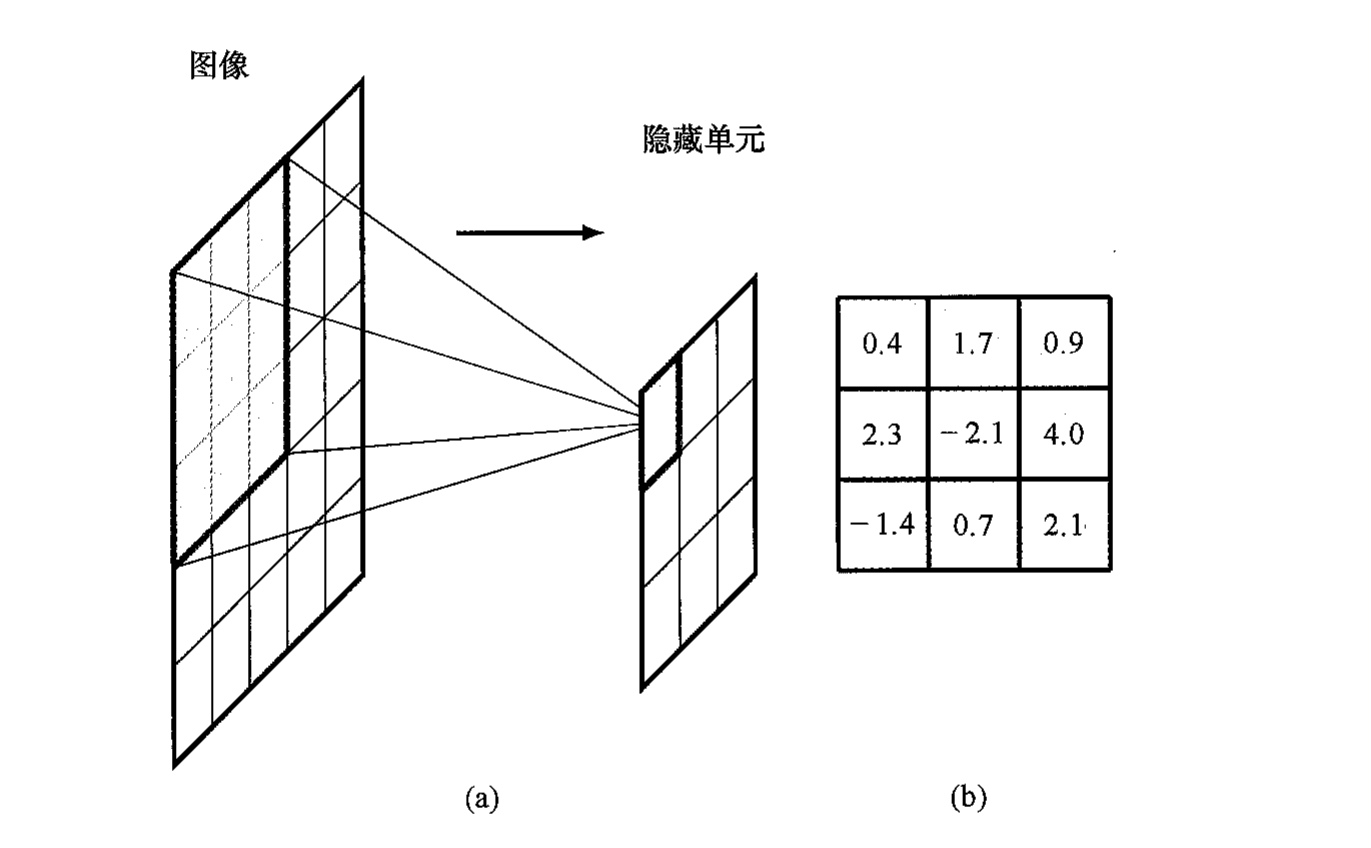
\includegraphics[width=0.78\textwidth]{ch10-fig10-1-感受野.png}
  \caption{感受野的图示。这里显示了网络隐藏层中的一个单元，该隐藏单元接收来自图像的 $3\times 3$ 小块像素输入，此小块中的像素构成了该隐藏单元的感受野。(b) 与该隐藏单元相关的权重值可以可视化为一个小的 $3\times 3$ 矩阵，称为卷积核。注意，还有一个额外的偏置参数，此处未显示。}
  \label{figure:ch10-感受野}
\end{figure}

假设\eqref{align:ch10-隐藏单元输出}中的 $\mathbf{w}$ 和 $w_0$ 是固定的，我们想知道对于哪一个输入图像小块 $\mathbf{x}$，这个隐藏单元将给出最大输出响应。为了回答这个问题，我们需要以某种方式约束 $\mathbf{x}$。假设它的范数 $\|\mathbf{x}\|^2$ 是固定的，那么对于某个系数 $\alpha$，使 $\mathbf{w}^{\mathsf{T}}\mathbf{x}$ 最大化并因此最大化隐藏单元响应的 $\mathbf{x}$ 的解的形式为 $\mathbf{x}=\alpha\mathbf{w}$（见\cref{exercise:ch10-01}）。也就是说，当检测到一个在整体缩放下像核图像的图像小块时，就会产生来自这个隐藏单元的最大输出响应。注意，只有当 $\mathbf{w}^{\mathsf{T}}\mathbf{x}$ 超过 $-w_0$ 的阈值时，ReLU 才会生成非零输出。因此该隐藏单元充当了特征检测器的角色，它会在找到与其卷积核匹配足够好的图像小块时发出信号。

\begin{proposition}[最大响应方向]\label{proposition:ch10-最大响应方向}
设 $\mathbf{w}\in\mathbb{R}^{n}$ 非零，$c>0$，在约束 $\|\mathbf{x}\|^2=c$ 下考虑函数 $f(\mathbf{x})=\mathbf{w}^{\mathsf{T}}\mathbf{x}$。则 $f$ 在约束集上的最大值在 $\mathbf{x}=\alpha\mathbf{w}$ 处取得，其中 $\alpha=\sqrt{c}/\|\mathbf{w}\|$；若 $\alpha$ 可取任意实数，则所有满足 $\mathbf{x}=\alpha\mathbf{w}$（$\alpha>0$）的点都是最大值点。
\end{proposition}
\begin{proof}
由 Cauchy-Schwarz 不等式，对任意满足 $\|\mathbf{x}\|^2=c$ 的 $\mathbf{x}$ 有
\begin{align*}
  \mathbf{w}^{\mathsf{T}}\mathbf{x}\leqslant \|\mathbf{w}\|\,\|\mathbf{x}\|=\|\mathbf{w}\|\sqrt{c}.
\end{align*}
取 $\mathbf{x}=\alpha\mathbf{w}$、$\alpha=\sqrt{c}/\|\mathbf{w}\|$，则 $\|\mathbf{x}\|^2=\alpha^2\|\mathbf{w}\|^2=c$，且
\begin{align*}
  \mathbf{w}^{\mathsf{T}}\mathbf{x}=\alpha\|\mathbf{w}\|^2=\sqrt{c}\,\|\mathbf{w}\|,
\end{align*}
故上界可取到。Cauchy-Schwarz 不等式的等号成立条件恰为 $\mathbf{x}$ 与 $\mathbf{w}$ 共线且同向，即 $\mathbf{x}=\alpha\mathbf{w}$，$\alpha>0$。当 $\alpha$ 可在实数中任取时，$\alpha>0$ 的共线点都取到同一个最大值 $\sqrt{c}\|\mathbf{w}\|$。证毕。
\end{proof}

% SUPPLEMENT: parent=proposition:ch10-最大响应方向; kind=motivation; location=紧随其后的 remark（重构新增）
\begin{remark}（重构新增）
这个命题说明了“隐藏单元是特征检测器”的精确含义：在输入能量固定的条件下，单元响应最大的输入小块恰是滤波器本身的一个正倍数。条件 $\|\mathbf{x}\|^2=c$ 不能去掉：若 $\mathbf{x}$ 可任意放大，$\mathbf{w}^{\mathsf{T}}\mathbf{x}$ 无上界，最大值不存在，“最匹配的小块”也就无从谈起。$\alpha>0$ 也不可换成 $\alpha\neq0$：$\mathbf{x}=-\alpha\mathbf{w}$ 给出的是最小响应，它对应“与核反相”的小块。命题只处理预激活 $\mathbf{w}^{\mathsf{T}}\mathbf{x}+w_0$；由于 ReLU 单调不减，最大化预激活与最大化 ReLU 输出等价。但“何时输出非零”由阈值决定：仅当 $\mathbf{w}^{\mathsf{T}}\mathbf{x}>-w_0$ 时才有非零响应，故偏置 $w_0$ 控制着检测器的触发门限，而不是匹配的方向。
\end{remark}

\subsection{平移等变性}\label{subsection:ch10-平移等变性}

接下来请注意，如果人脸图像中的小块表示处在该位置的眼睛，那么图像不同部分的同一组像素值表示新位置的眼睛。我们的神经网络需要能够将其在一个位置学到的知识泛化到图像中的所有可能位置，而不需要在训练集中每个可能位置见过对应特征的示例。为了实现这一点，我们可以简单地在图像的多个位置复制相同的隐藏单元权值，如\cref{figure:ch10-一维卷积}中的一维输入空间所示。

隐藏层的单元形成一个特征图（feature map），其中，所有单元共享相同的权重。因此，如果图像的局部小块在连接到该小块的单元中产生特定响应，则不同位置的同一组像素值将在特征图中的相应变换位置产生相同的响应。这是等变性（equivariance）的一个例子（参见\cref{subsection:ch09-等变性}）。可以看到这个网络中的连接是稀疏的（sparse），因为大多数连接不存在。此外，权值由所有隐藏单元共享，如连接的颜色所示。这一变换是卷积（convolution）的一个例子。

\begin{figure}[htbp]
  \centering
  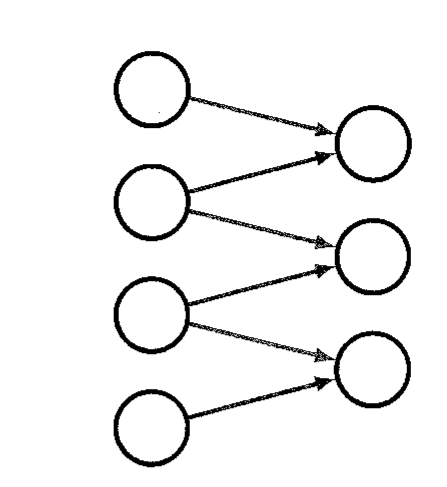
\includegraphics[width=0.42\textwidth]{ch10-fig10-2-一维卷积.png}
  \caption{输入值的一维数组以及宽度为 2 的核卷积示意图。连接是稀疏的，由隐藏单元共享，如红色和蓝色箭头所示，其中具有相同颜色的连接具有相同的权值。因此，该网络有 6 个连接，但只有两个独立的学习参数。}
  \label{figure:ch10-一维卷积}
\end{figure}

我们可以将卷积的想法扩展到二维图像（Dumoulin and Visin, 2016）。对于像素强度为 $I(j,k)$ 的图像 $I$ 和像素值为 $K(l,m)$ 的滤波器 $K$，特征图 $C$ 的激活值由下式给出：
\begin{align}
  C(j,k) = \sum_{l}\sum_{m} I(j+l,\,k+m)\,K(l,m).
  \label{align:ch10-二维卷积}
\end{align}

\begin{definition}[特征图]\label{definition:ch10-特征图}
设一层中若干隐藏单元以相同方式作用于输入的不同空间位置，则称这些单元的激活值按空间位置排成的二维数组为该层的\textbf{特征图}（feature map）。特征图中所有单元共享同一组权重；若一层有多个特征图，则称每个特征图为该层的一个\textbf{通道}（channel）。
\end{definition}

% SUPPLEMENT: parent=definition:ch10-特征图; kind=motivation; location=紧随其后的 remark（重构新增）
\begin{remark}（重构新增）
特征图把“位置”与“内容”分开存放：数组的两个下标是位置，数组元素是内容。定义中“以相同方式作用”就是权重共享，它是等变性（\cref{proposition:ch10-平移等变性}）成立的结构性前提；如果不同位置使用不同权重，同一小块像素平移到新位置后响应会改变，等变性立即失效。把多个特征图称为通道，是为了与图像的 RGB 通道使用同一套张量语言，从而让\cref{definition:ch10-多维卷积}中的四阶滤波器张量有意义。注意特征图是“对一幅输入图像的一层输出”，不是网络的参数，也不参与训练。
\end{remark}

\begin{definition}[卷积（互相关）]\label{definition:ch10-卷积}
设 $I$ 为 $J\times K$ 的图像，$K$ 为 $M\times M$ 的滤波器。称由\eqref{align:ch10-二维卷积}定义的数组 $C$ 为 $I$ 与 $K$ 的\textbf{卷积}，并记 $C=I*K$。严格地说，\eqref{align:ch10-二维卷积}实现的是\textbf{互相关}（cross-correlation）；机器学习文献惯例上仍称之为卷积。
\end{definition}

% SUPPLEMENT: parent=definition:ch10-卷积; kind=motivation; location=紧随其后的 remark（重构新增）
\begin{remark}（重构新增）
这个定义有两处需要说明。第一，求和范围由“滤波器完全落在图像内”决定，即 $l,m$ 取使 $1\leqslant j+l\leqslant J$、$1\leqslant k+m\leqslant K$ 的全部整数，故 $C$ 的尺寸比 $I$ 小（\cref{proposition:ch10-填充输出尺寸}将精确写出）。第二，互相关与数学上的卷积相差一次核翻转（见\cref{exercise:ch10-04}），但在卷积网络中滤波器是学习得到的，翻转与否只是把参数重新编号，不改变模型族，因此沿用“卷积”这一名称不会损失任何表达能力。真正重要的是公式中的两个性质：对 $l,m$ 求和使输出对输入的局部平移等变，系数 $K(l,m)$ 与 $j,k$ 无关使权重在所有位置共享。
\end{remark}

\begin{proposition}[卷积的平移等变性]\label{proposition:ch10-平移等变性}
设 $I$ 为图像，$K$ 为 $M\times M$ 滤波器，$C=I*K$ 由\eqref{align:ch10-二维卷积}给出，且不施加边界填充（即只对使滤波器完全落在图像内的位置定义 $C$）。对整数 $\delta_j,\delta_k$，定义平移算子 $(T_{\delta_j,\delta_k}I)(j,k)=I(j-\delta_j,k-\delta_k)$。则在两边都有定义的位置上成立
\begin{align}
  \bigl(T_{\delta_j,\delta_k}I\bigr)*K = T_{\delta_j,\delta_k}\bigl(I*K\bigr).
  \label{align:ch10-平移等变性}
\end{align}
即卷积与平移可交换：输入平移多少，特征图就在相同方向上平移多少。
\end{proposition}
\begin{proof}
记 $\tilde{I}=T_{\delta_j,\delta_k}I$，即 $\tilde{I}(j,k)=I(j-\delta_j,k-\delta_k)$。按\eqref{align:ch10-二维卷积}，
\begin{align*}
  \bigl(\tilde{I}*K\bigr)(j,k)=\sum_{l}\sum_{m}\tilde{I}(j+l,k+m)K(l,m)
  =\sum_{l}\sum_{m}I(j-\delta_j+l,\,k-\delta_k+m)K(l,m).
\end{align*}
另一方面，令 $j'=j-\delta_j$、$k'=k-\delta_k$，由同一公式
\begin{align*}
  \bigl(I*K\bigr)(j',k')=\sum_{l}\sum_{m}I(j'+l,\,k'+m)K(l,m),
\end{align*}
故 $\bigl(\tilde{I}*K\bigr)(j,k)=\bigl(I*K\bigr)(j-\delta_j,k-\delta_k)=\bigl(T_{\delta_j,\delta_k}(I*K)\bigr)(j,k)$。由于 $j,k$ 任意，\eqref{align:ch10-平移等变性}成立。证毕。
\end{proof}

% SUPPLEMENT: parent=proposition:ch10-平移等变性; kind=motivation; location=紧随其后的 remark（重构新增）
\begin{remark}（重构新增）
等变（equivariance）与不变（invariance）是两件不同的事，这个命题给出的是前者：输出随输入一起平移，而不是保持不变。条件“不施加边界填充”只是为了回避边界效应：在补零填充下，靠近边界的位置会看到人为的零，平移后看到的零的个数改变，等式只在离开边界足够远的位置成立。这正是卷积网络需要\cref{definition:ch10-填充}的原因之一，也是池化（\cref{definition:ch10-池化}）之后才能得到近似平移不变性的原因。命题对任意滤波器成立，与 $K$ 的取值无关，因此等变性是架构的性质而非学习的结果；网络中真正从数据中学到的是“检测什么特征”，而不是“是否等变”。
\end{remark}

通过将这种卷积结构与标准的全连接网络作比较，我们看到了前者的 3 个优点：首先，连接是稀疏的，即使对于较大的图像，权重也要少得多；其次，权值是共享的，这大大减少了独立参数的数量，从而减小了学习这些参数所需的训练集大小；最后，相同的网络可以应用于不同大小的图像，而无需重新训练。我们稍后将重新讨论最后一点，但目前，你只需要注意，改变输入图像的大小只会更改特征图的大小，而不会改变模型中的权重数量或独立可学习参数的数量（参见\cref{subsection:ch10-滑动窗口}）。关于卷积网络的最后一个观察是，通过利用图形处理单元（Graphics Processing Unit, GPU）高计算吞吐量的大规模并行特性，卷积在实现中计算效率非常高。

\begin{figure}[htbp]
  \centering
  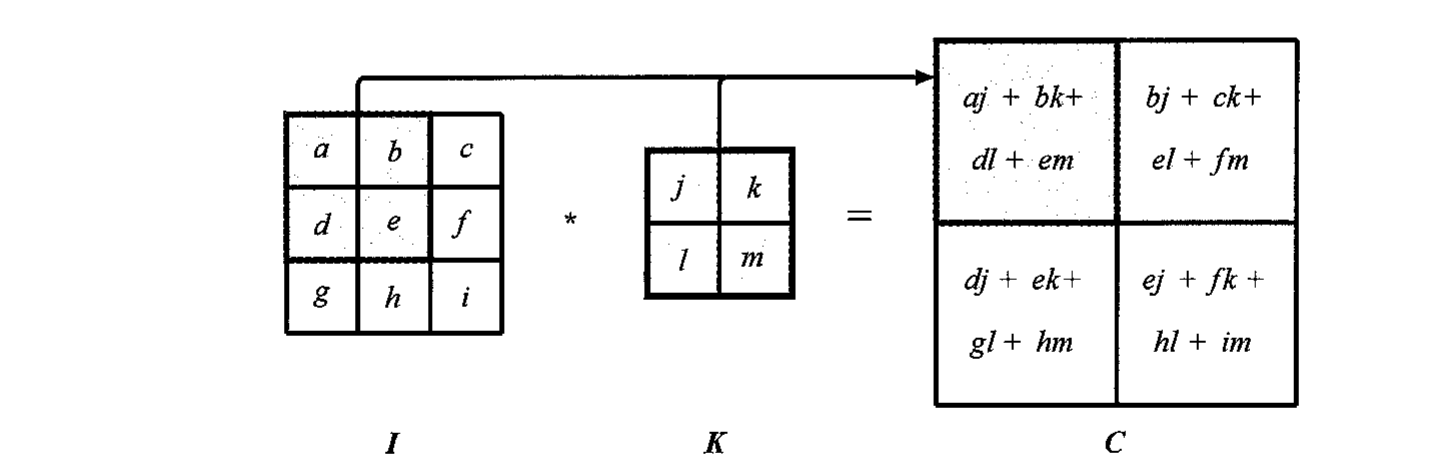
\includegraphics[width=0.72\textwidth]{ch10-fig10-3-二维卷积示例.png}
  \caption{在 $3\times 3$ 的图像上使用 $2\times 2$ 滤波器卷积的示例，以及得到的 $2\times 2$ 特征图。}
  \label{figure:ch10-二维卷积示例}
\end{figure}

作为卷积应用的一个例子，考虑使用固定的、手工制作的卷积滤波器检测图像边缘的问题。直观上，可以认为垂直边缘是我们在图像上水平移动时，因像素之间的强度发生显著的局部变化而产生的。我们可以通过使用以下形式的 $3\times 3$ 滤波器对图像进行卷积来测量这一点：
\begin{align}
  K = \begin{bmatrix} -1 & 0 & 1\\ -1 & 0 & 1\\ -1 & 0 & 1 \end{bmatrix}.
  \label{align:ch10-竖直边缘滤波器}
\end{align}
类似地，我们也可以使用此滤波器的转置来对图像进行卷积，从而检测图像的水平边缘：
\begin{align}
  K = \begin{bmatrix} -1 & -1 & -1\\ 0 & 0 & 0\\ 1 & 1 & 1 \end{bmatrix}.
  \label{align:ch10-水平边缘滤波器}
\end{align}
\cref{figure:ch10-边缘检测}显示了将这两个卷积滤波器应用于示例图像的结果。注意在\cref{figure:ch10-边缘检测}(b) 中，如果竖直边缘对应于像素强度的增加，则特征图上的相应点为正（用浅色表示）；而如果竖直边缘对应于像素强度的降低，则特征图上的相应点为负（用深色表示）。\cref{figure:ch10-边缘检测}(c) 所示水平边缘的结果具有类似的性质。

\begin{figure}[htbp]
  \centering
  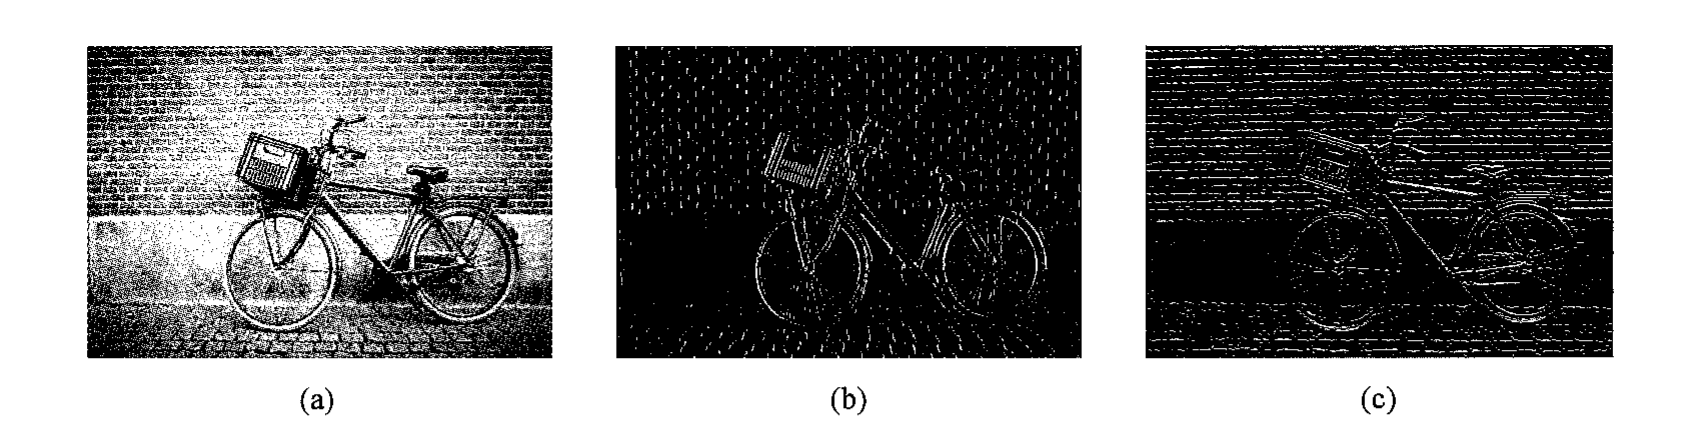
\includegraphics[width=0.95\textwidth]{ch10-fig10-4-边缘检测.png}
  \caption{使用卷积滤波器检测图像边缘的示意图：(a) 原始图像；(b) 使用滤波器\eqref{align:ch10-竖直边缘滤波器}卷积检测竖直边缘的结果；(c) 使用滤波器\eqref{align:ch10-水平边缘滤波器}卷积检测水平边缘的结果。}
  \label{figure:ch10-边缘检测}
\end{figure}

\subsection{填充}\label{subsection:ch10-填充}

从\cref{figure:ch10-二维卷积示例}中可以看出，卷积图比原始图像小。如果原始图像的维度为 $J\times K$，并且我们用维度为 $M\times M$ 的核对其进行卷积（滤波器通常是正方形的），则生成的特征图的维度为 $(J-M+1)\times (K-M+1)$。在某些情况下，我们希望特征图具有与原始图像相同的尺寸。这可以通过在原始图像外部填充（padding）额外像素来实现，如\cref{figure:ch10-填充示意}所示。如果我们用 $P$ 个像素填充原始图像，则输出的特征图的维度为 $(J+2P-M+1)\times (K+2P-M+1)$。如果没有对原始图像进行填充，即 $P=0$，则称为有效（valid）卷积。当选择的 $P$ 值使得输出数组的大小与输入数组的大小相同时，对应于 $P=(M-1)/2$，则称为等大（same）卷积，因为原始图像和特征图具有相同的维度（见\cref{exercise:ch10-06}）。在计算机视觉中，滤波器的 $M$ 通常为奇数，因此填充可以在原始图像的所有边上对称进行，并且滤波器具有一个与位置关联的明确定义的中心像素。最后，我们需要为填充像素选择一个合适的强度值。典型的选择是将填充值设置为零（在先从每个图像中减去平均值之后），这样零就是像素强度的平均值。填充也可以应用于特征图，以便由后续卷积层处理。

\begin{figure}[htbp]
  \centering
  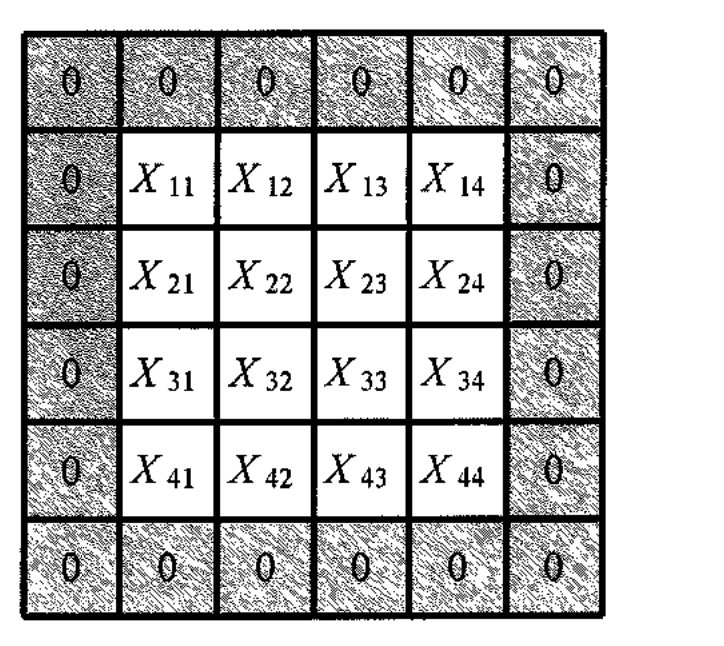
\includegraphics[width=0.42\textwidth]{ch10-fig10-5-填充示意.png}
  \caption{$4\times 4$ 图像的填充示意图，该图像已填充了额外像素以创建 $6\times 6$ 图像。}
  \label{figure:ch10-填充示意}
\end{figure}

\begin{definition}[填充、有效卷积与等大卷积]\label{definition:ch10-填充}
在图像（或特征图）的每条边外侧各补上 $P$ 个取固定值的像素，称为\textbf{填充}（padding），$P$ 称为填充宽度。若 $P=0$，称相应的卷积为\textbf{有效}（valid）卷积；若 $P=(M-1)/2$（$M$ 为奇数），称相应的卷积为\textbf{等大}（same）卷积。填充值通常取 $0$，且取零之前先从每幅图像中减去像素强度的均值。
\end{definition}

% SUPPLEMENT: parent=definition:ch10-填充; kind=motivation; location=紧随其后的 remark（重构新增）
\begin{remark}（重构新增）
填充的唯一目的是控制输出尺寸，但它同时改变了边界处看到的内容：位于边界附近的单元在原图上只有半个感受野，补零后它“看到”的是人为的零，这与图像内部单元看到的统计量并不一致。于是“先减去均值再补零”成为一个有实质内容的约定：若像素均值不为零而直接补零，边界单元会持续收到一个偏置信号，等变性\eqref{align:ch10-平移等变性}在边界附近被破坏得更严重。$P=(M-1)/2$ 只对奇数 $M$ 给出整数，这也是计算机视觉中滤波器尺寸常取奇数的原因之一；若 $M$ 为偶数，对称填充无法使输出与输入同尺寸。注意“等大卷积”不改变参数量，只是让空间分辨率得以在深层网络中保持。
\end{remark}

\begin{proposition}[填充卷积的输出尺寸]\label{proposition:ch10-填充输出尺寸}
设输入为 $J\times K$，滤波器为 $M\times M$，填充宽度为 $P$，步幅为 $1$。则输出特征图的尺寸为
\begin{align}
  (J+2P-M+1)\times(K+2P-M+1).
  \label{align:ch10-填充输出尺寸}
\end{align}
特别地，当 $M$ 为奇数且 $P=(M-1)/2$ 时输出尺寸等于输入尺寸 $J\times K$。
\end{proposition}
\begin{proof}
填充后数组的边长为 $J+2P$ 与 $K+2P$。滤波器在水平方向可放置的位置数为 $(J+2P)-M+1$：第一个位置使滤波器的第 $1$ 列对齐填充数组的第 $1$ 列，最后一个位置使滤波器的第 $M$ 列对齐填充数组的第 $J+2P$ 列，中间每个整数偏移给出一个位置，故共有 $J+2P-M+1$ 个。竖直方向同理为 $K+2P-M+1$。每个位置对应输出特征图的一个元素，故\eqref{align:ch10-填充输出尺寸}成立。取 $P=(M-1)/2$ 得 $J+2P-M+1=J+(M-1)-M+1=J$，竖直方向同理。证毕。
\end{proof}

% SUPPLEMENT: parent=proposition:ch10-填充输出尺寸; kind=motivation; location=紧随其后的 remark（重构新增）
\begin{remark}（重构新增）
这个公式是后面所有尺寸计算的基石，使用时要注意三点。第一，它要求 $J+2P\geqslant M$，否则滤波器放不进填充后的数组，输出尺寸为零或负，卷积无定义。第二，公式对特征图同样适用，只需把 $J,K$ 换成上一层的输出尺寸，这正是逐层追踪网络形状的依据。第三，等大填充保持的是空间尺寸而不是信息量：边界处的输出仍由补出来的零参与计算，因此“输出与输入同尺寸”不等于“边界处理无损失”。
\end{remark}

\subsection{跨步卷积}\label{subsection:ch10-跨步卷积}

在典型的图像处理应用中，图像可以有非常多的像素，并且由于卷积核通常相对较小，因此 $M\ll J,K$，特征图的大小将与原始图像相似（如果进行等大填充，则大小相同）。有时，我们希望使用比原始图像小得多的特征图，以便在设计卷积网络时更灵活。实现此目的的一种方法是使用跨步卷积（strided convolution），即不再将滤波器一次移动一个像素，而是以较大的步长 $S$ 移动滤波器。我们称 $S$ 为步幅（stride）。如果在水平和竖直方向上使用相同的步幅，那么特征图中的元素数量为（见\cref{exercise:ch10-07}）：
\begin{align}
  \left\lfloor \frac{J+2P-M}{S}+1\right\rfloor
  \times
  \left\lfloor \frac{K+2P-M}{S}+1\right\rfloor,
  \label{align:ch10-跨步卷积输出尺寸}
\end{align}
其中 $\lfloor x\rfloor$ 表示将 $x$ 向下取整，得到小于或等于 $x$ 的最大整数。对于大图像和小尺寸滤波器，特征图将是原始图像大小的 $1/S$。

\begin{definition}[跨步卷积与步幅]\label{definition:ch10-跨步卷积}
在卷积中，若滤波器每次沿水平或竖直方向移动 $S$ 个像素而不是 $1$ 个像素，则称该运算为\textbf{跨步卷积}（strided convolution），称 $S$ 为\textbf{步幅}（stride）。若两个方向使用相同的步幅，则称步幅为 $S$。
\end{definition}

% SUPPLEMENT: parent=definition:ch10-跨步卷积; kind=motivation; location=紧随其后的 remark（重构新增）
\begin{remark}（重构新增）
步幅提供了一种与池化不同的下采样手段：它不引入任何额外的池化参数，而是在卷积本身中跳着取样。定义要求 $S$ 为正整数，因为滤波器位置必须落在像素网格上；$S=1$ 退化为普通卷积。步幅带来的代价是信息丢失的不可逆性：被跳过的位置完全不参与输出，这一点与池化相同，但跨步卷积同时仍在做特征变换，因此它在降分辨率的同时保留了“学到的”表示，而池化只做固定的聚合。步幅与填充是两套独立机制，前者控制采样密度，后者控制边界。
\end{remark}

\begin{proposition}[跨步卷积的输出尺寸]\label{proposition:ch10-跨步卷积输出尺寸}
设输入为 $J\times K$，滤波器为 $M\times M$，填充宽度为 $P$，步幅为 $S$，且 $J+2P\geqslant M$、$K+2P\geqslant M$。则输出特征图的尺寸由\eqref{align:ch10-跨步卷积输出尺寸}给出。
\end{proposition}
\begin{proof}
考察水平方向。填充后数组长度为 $J+2P$。滤波器的左端位置依次为 $0,S,2S,\cdots$，第 $t$ 个位置（$t=0,1,2,\cdots$）要求滤波器完全落在数组内，即 $tS+M\leqslant J+2P$，等价于 $t\leqslant (J+2P-M)/S$。满足该不等式的非负整数 $t$ 的个数为 $\lfloor (J+2P-M)/S\rfloor+1$，这正是输出特征图的列数。竖直方向同理给出 $\lfloor (K+2P-M)/S\rfloor+1$ 行。两方向独立，故总元素个数为二者之积。当 $J,K\gg M$ 且 $P$ 相对 $J,K$ 可忽略时，该数约为 $J/S$ 与 $K/S$，即特征图边长约为原图的 $1/S$。证毕。
\end{proof}

% SUPPLEMENT: parent=proposition:ch10-跨步卷积输出尺寸; kind=motivation; location=紧随其后的 remark（重构新增）
\begin{remark}（重构新增）
向下取整是公式的要害：它说明当 $(J+2P-M)$ 不能被 $S$ 整除时，最后一段像素被丢弃，输出尺寸不是简单的除法。若把 $S$ 增大而不同时调整 $P$，可能出现某个位置被完全跳过、或边界像素从未被任何滤波器位置覆盖的情形，因此实际实现中常配合 $P$ 使 $J+2P-M$ 尽量被 $S$ 整除。条件 $J+2P\geqslant M$ 不可省，否则连第一个位置都放不下。公式对多层网络逐层使用即可追踪形状，这一点在\cref{proposition:ch10-有效感受野}中还会用到。
\end{remark}

\subsection{多维卷积}\label{subsection:ch10-多维卷积}

到目前为止，我们已经考虑了单个灰度图像上的卷积。彩色图像有三个通道，对应于红色、绿色和蓝色。通过扩展滤波器的维度，我们可以轻松地扩展卷积以支持多个通道。具有 $J\times K$ 个像素和 $C$ 个通道的图像可以用维度为 $J\times K\times C$ 的张量来描述（参见\cref{section:ch06-深度网络}）。我们可以引入一个用维度为 $M\times M\times C$ 的张量来描述的滤波器，该张量对于 $C$ 个通道中的每一个通道，都有一个独立的 $M\times M$ 滤波器。假设对原始图像没有进行填充且步幅为 1，则同样可以得到大小为 $(J-M+1)\times (K-M+1)$ 的特征图，如\cref{figure:ch10-多维卷积}所示。

\begin{definition}[多通道卷积与通道数]\label{definition:ch10-多维卷积}
设输入张量为 $I\in\mathbb{R}^{J\times K\times C_{\mathrm{in}}}$，滤波器张量为 $W\in\mathbb{R}^{M\times M\times C_{\mathrm{in}}\times C_{\mathrm{out}}}$。对 $c=1,\cdots,C_{\mathrm{out}}$，定义第 $c$ 个输出通道为
\begin{align}
  O_c(j,k)=\sum_{c'=1}^{C_{\mathrm{in}}}\sum_{l}\sum_{m} I_{c'}(j+l,\,k+m)\,W(l,m,c',c)+b_c,
  \label{align:ch10-多通道卷积}
\end{align}
其中 $b_c$ 为第 $c$ 个输出通道的偏置，$I_{c'}$ 表示输入的第 $c'$ 个通道。称 $C_{\mathrm{in}}$ 为输入通道数，$C_{\mathrm{out}}$ 为输出通道数，称 $O_1,\cdots,O_{C_{\mathrm{out}}}$ 为输出的各个通道。
\end{definition}

% SUPPLEMENT: parent=definition:ch10-多维卷积; kind=motivation; location=紧随其后的 remark（重构新增）
\begin{remark}（重构新增）
这个定义把“在每个输入通道上各有一个 $M\times M$ 滤波器”与“把各通道的结果相加”两件事合成一个张量运算：滤波器张量的最后一维 $C_{\mathrm{out}}$ 取不同值时，取到的是完全独立的一组 $C_{\mathrm{in}}$ 个二维滤波器。求和指标 $c'$ 遍历全部输入通道而不是某一个，因此单个输出通道看到的是所有输入通道的联合信息，这正是彩色图像第一层能检测“颜色-方向”组合特征的原因。若去掉对 $c'$ 的求和、只保留单通道，就退化为一维卷积在通道上的堆叠，各通道之间不再交互，表达能力显著下降。
\end{remark}

\begin{figure}[htbp]
  \centering
  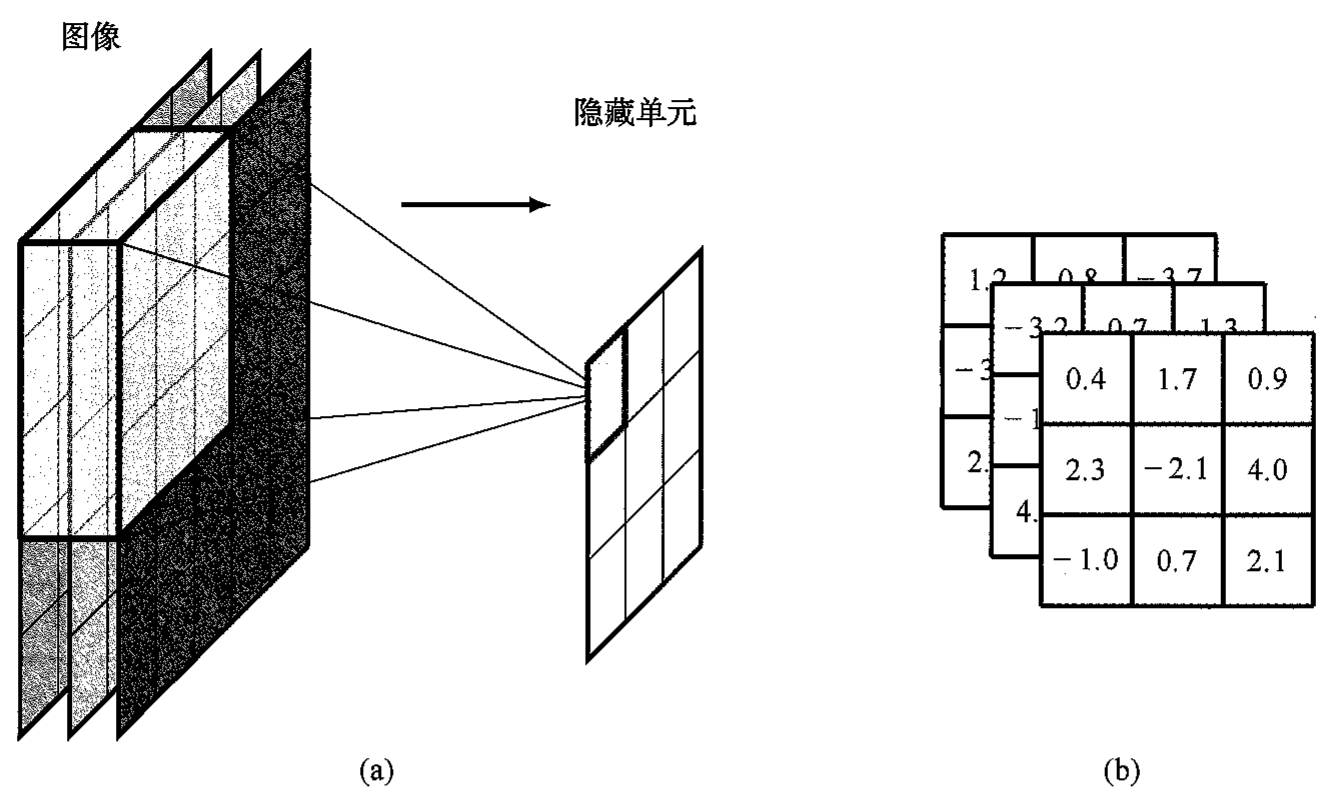
\includegraphics[width=0.9\textwidth]{ch10-fig10-6-多维卷积.png}
  \caption{(a) 从 R、G 和 B 通道接收输入的多维滤波器示意图；(b) 这里的核有 27 个权重（加上 1 个未显示的偏置参数），它可以可视化为一个 $3\times 3\times 3$ 大小的张量。}
  \label{figure:ch10-多维卷积}
\end{figure}

下面让我们对卷积进一步进行重要扩展。目前，我们已经创建了单一的特征图，并且特征图中的所有点共享同一组可学习参数。对于维度为 $M\times M\times C$ 的滤波器，无论图像大小如何，都将有 $M^2C$ 个权重参数。此外，还有一个与该单元相关的偏置参数。这种滤波器类似于全连接网络中的单个隐藏节点，它只能学习检测一种特征，因此作用非常有限。为了构建更灵活的模型，我们需要使用多个这样的滤波器，其中每个滤波器都有互不相关的参数集，从而产生独立的特征图，如\cref{figure:ch10-多通道卷积}所示。我们再次将这些独立的特征图称为通道（channel）。滤波器张量现在的维度为 $M\times M\times C\times C_{\mathrm{out}}$，其中 $C$ 是输入通道数，$C_{\mathrm{out}}$ 是输出通道数。每个输出通道都有自己的相关偏置参数，因此参数总数为 $(M^2C+1)C_{\mathrm{out}}$。

\begin{figure}[htbp]
  \centering
  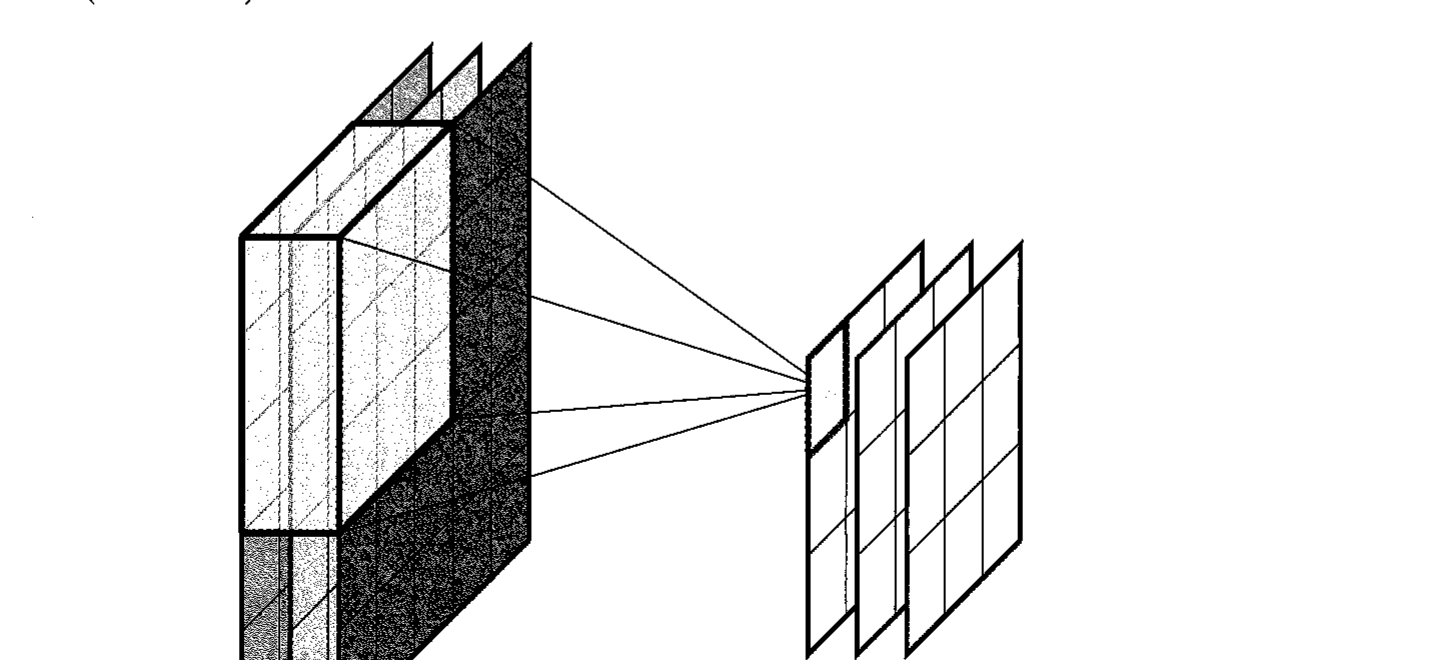
\includegraphics[width=0.85\textwidth]{ch10-fig10-7-多通道卷积.png}
  \caption{\cref{figure:ch10-多维卷积}所示的多维卷积滤波层可以扩展为包括多个独立的滤波通道。}
  \label{figure:ch10-多通道卷积}
\end{figure}

\begin{proposition}[卷积层参数量]\label{proposition:ch10-卷积层参数量}
设一个卷积层的输入有 $C_{\mathrm{in}}$ 个通道，滤波器空间尺寸为 $M\times M$，输出有 $C_{\mathrm{out}}$ 个通道，每个输出通道带一个偏置。则该层的可学习参数总数为
\begin{align}
  \bigl(M^2C_{\mathrm{in}}+1\bigr)C_{\mathrm{out}}.
  \label{align:ch10-卷积层参数量}
\end{align}
该数目与输入的空间尺寸 $J\times K$ 无关；该层的连接数为 $M^2C_{\mathrm{in}}C_{\mathrm{out}}J'K'$，其中 $J'\times K'$ 为输出特征图的空间尺寸。
\end{proposition}
\begin{proof}
由\cref{definition:ch10-多维卷积}，第 $c$ 个输出通道用到权重 $W(\cdot,\cdot,\cdot,c)$，共 $M\cdot M\cdot C_{\mathrm{in}}=M^2C_{\mathrm{in}}$ 个，再加一个偏置 $b_c$，故每个输出通道有 $M^2C_{\mathrm{in}}+1$ 个参数。$C_{\mathrm{out}}$ 个输出通道的参数集互不相关，故总数为 $(M^2C_{\mathrm{in}}+1)C_{\mathrm{out}}$。该表达式不含 $J,K$，故与输入空间尺寸无关。连接数方面，输出特征图的每个元素通过 $M^2C_{\mathrm{in}}$ 条边连到输入，输出元素共 $J'K'C_{\mathrm{out}}$ 个，故连接总数为 $M^2C_{\mathrm{in}}C_{\mathrm{out}}J'K'$。证毕。
\end{proof}

% SUPPLEMENT: parent=proposition:ch10-卷积层参数量; kind=motivation; location=紧随其后的 remark（重构新增）
\begin{remark}（重构新增）
这个命题量化了\cref{section:ch10-卷积滤波器}开头关于参数量的对比：第一层 $3\times 3$、$C_{\mathrm{in}}=3$、$C_{\mathrm{out}}=64$ 的卷积层只有 $(9\cdot3+1)\cdot64=1792$ 个参数，而同尺寸输入上的全连接层需要 $10^6\cdot 3\cdot 1000$ 量级的权重。注意“参数少”与“连接多”并不矛盾：连接数仍与空间尺寸成正比（乘上了 $J'K'$），减少的是独立自由度而非计算量。条件“每个输出通道带一个偏置”是本书采用的约定；若某些实现共享偏置或使用无偏置卷积，公式相应变为 $M^2C_{\mathrm{in}}C_{\mathrm{out}}$ 或 $M^2C_{\mathrm{in}}C_{\mathrm{out}}+C_{\mathrm{out}}$，这不影响数量级结论。
\end{remark}

设计卷积网络时的一个有用概念是 $1\times 1$ 卷积（Lin, Chen, and Yan, 2013），它是一个滤波器大小为单个像素的卷积层。滤波器有 $C$ 个权重（每个输入通道一个权重），外加一个偏置。$1\times 1$ 卷积通过将输出通道数设置为与输入通道数不同，可以简单地用来改变通道数（通常用来减少通道数），而不改变特征图的大小。因此，它是对跨步卷积或池化的补充，因为它减少了通道的数量而不是通道的维度。

\begin{definition}[$1\times 1$ 卷积]\label{definition:ch10-1x1卷积}
称空间尺寸为 $1\times 1$ 的卷积为 $1\times 1$ \textbf{卷积}，即对每个空间位置 $(j,k)$ 独立地施加同一个线性映射
\begin{align}
  O_c(j,k)=\sum_{c'=1}^{C_{\mathrm{in}}} W(1,1,c',c)\,I_{c'}(j,k)+b_c,\qquad c=1,\cdots,C_{\mathrm{out}}.
  \label{align:ch10-1x1卷积}
\end{align}
\end{definition}

% SUPPLEMENT: parent=definition:ch10-1x1卷积; kind=motivation; location=紧随其后的 remark（重构新增）
\begin{remark}（重构新增）
$1\times 1$ 卷积是“逐像素的全连接层”：它在每个空间位置上使用同一组权重，因而完全不看邻域，只做通道间的线性混合。它的参数量为 $(C_{\mathrm{in}}+1)C_{\mathrm{out}}$，与空间尺寸无关，因此常被用来在不改变分辨率的前提下压缩或扩展通道数，例如在 U-Net 的最后一层把通道数降到类别数（\cref{subsection:ch10-U-Net架构}）。把它与\cref{definition:ch10-多维卷积}比较可以看出，它只是 $M=1$ 的特例，并不是新的运算；把它单列出来是因为它在网络设计中承担“通道变换”这一独立职能。若在 $1\times 1$ 卷积后再接非线性激活，它就成为逐像素的两层感知机。
\end{remark}

\subsection{池化}\label{subsection:ch10-池化}

卷积层编码了平移等变性（equivariance）：如果将一小块像素（代表隐藏单元的感受野）移动到图像中的不同位置，则特征图的关联输出将移动到特征图中的相应位置。这对于在图像中找到目标的位置等应用很有价值。对于其他应用，例如图像分类，我们希望在输入平移时，输出保持不变。然而，在所有情况下，我们都希望网络能够学习分层结构，其中特定级别的复杂特征是由前一级的简单特征构建而成的。在许多情况下，这些简单特征之间的空间关系非常重要。例如，眼睛、鼻子和嘴巴的相对位置有助于确定面部的存在，而非仅仅表明这些特征在图像中存在。但是，相对位置的微小变化不会影响分类，我们希望对单个特征的这种小平移保持输出不变。这可以通过在卷积层输出之后，应用池化（pooling）来实现。

池化与卷积有相似之处，因为单元阵列排列在网格中，且其中的每个单元都从前一个特征图的感受野中获取输入。此外，池化同样需要选择滤波器大小和步幅。然而，池化与卷积的不同之处在于，池化单元的输出是其输入的简单、固定的函数，因此池化中没有可学习参数。池化的一个常见示例是最大池化（max-pooling）（Zhou and Chellappa, 1988），其中每个单元仅输出对于输入值的“取最大值”函数。\cref{figure:ch10-最大池化}所示的简单示例说明了这一过程。这里的步幅等于滤波器的宽度，因此感受野没有重叠。

\begin{definition}[池化与最大池化]\label{definition:ch10-池化}
设特征图为 $A$，池化窗口为 $M\times M$、步幅为 $S$。若池化单元的输出为窗口内全部输入值的最大值，则称该运算为\textbf{最大池化}（max-pooling）；若为窗口内全部输入值的平均值，则称\textbf{平均池化}（average pooling）。池化不含可学习参数，且通常对每个通道独立施加。
\end{definition}

% SUPPLEMENT: parent=definition:ch10-池化; kind=motivation; location=紧随其后的 remark（重构新增）
\begin{remark}（重构新增）
池化把“特征是否存在”与“特征在哪里”分开：最大池化保留窗口内的最大响应（存在性与强度），但丢弃最大值的位置（位置信息）。这正是它在图像分类中有用、在语义分割中却造成麻烦的原因（\cref{subsection:ch10-U-Net架构}）。定义强调“对每个通道独立施加”，否则不同通道的响应会被混在一起，通道语义被破坏；也强调“无可学习参数”，因此池化不增加模型容量，只改变表示。窗口与步幅都等于 $M$ 时窗口互不重叠，输出尺寸恰为输入的 $1/M$；若步幅小于窗口，则窗口重叠，输出更大但仍小于输入。
\end{remark}

\begin{figure}[htbp]
  \centering
  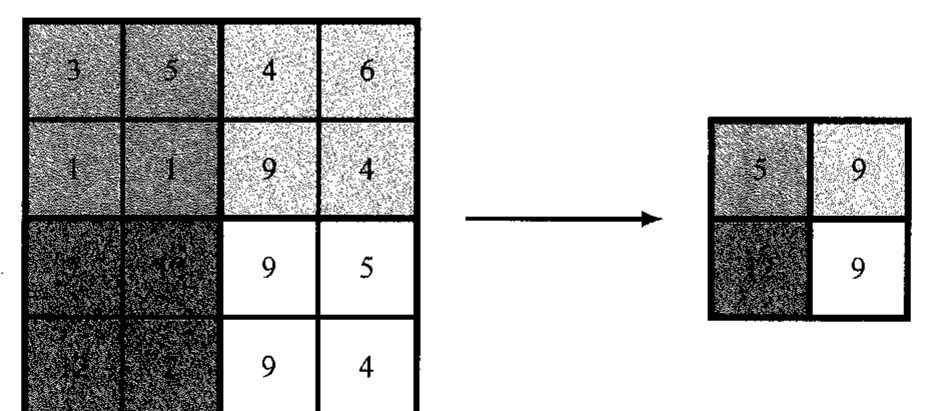
\includegraphics[width=0.62\textwidth]{ch10-fig10-8-最大池化.png}
  \caption{最大池化示意图，其中使用“max”运算符将特征图中的 $2\times 2$ 像素块组合在一起，从而生成较小维度的新特征图。}
  \label{figure:ch10-最大池化}
\end{figure}

除了构建一些局部平移不变性外，池化通过对特征图下采样，还可用于降低表示的维度。注意，在卷积层中使用大于 1 的步幅也可以实现对特征图下采样的效果。

我们可以将特征图中单元的激活解释为检测相应特征强度的度量，因此最大池化保留了有关特征是否存在以及特征强度的信息，但丢弃了一些位置信息。池化还有许多其他选择，例如平均池化（average pooling），其中池化函数计算特征图中相应感受野值的平均值。这些都引入了一定程度的局部平移不变性。

\begin{proposition}[池化的输出尺寸与局部不变性]\label{proposition:ch10-池化输出尺寸}
设特征图的空间尺寸为 $J\times K$，池化窗口为 $M\times M$、步幅为 $S$。则池化输出的空间尺寸为
\begin{align}
  \left\lfloor\frac{J-M}{S}\right\rfloor+1
  \;\times\;
  \left\lfloor\frac{K-M}{S}\right\rfloor+1 .
  \label{align:ch10-池化输出尺寸}
\end{align}
当 $S=M$ 时输出尺寸为 $\lfloor J/M\rfloor\times\lfloor K/M\rfloor$，即窗口互不重叠。此外，若输入在窗口内发生不超过窗口范围的平移，且窗口内最大值唯一，则最大池化的输出在相应窗口内保持不变。
\end{proposition}
\begin{proof}
尺寸公式与\cref{proposition:ch10-跨步卷积输出尺寸}在 $P=0$ 时的情形完全相同：窗口左端可放置的位置为 $0,S,2S,\cdots$，第 $t$ 个位置要求 $tS+M\leqslant J$，故 $t\leqslant (J-M)/S$，位置个数为 $\lfloor (J-M)/S\rfloor+1$。取 $S=M$ 得 $\lfloor (J-M)/M\rfloor+1=\lfloor J/M\rfloor$（当 $J$ 为 $M$ 的整数倍时等号成立，一般情形由取整给出）。关于不变性：设某窗口内的输入为 $a_1,\cdots,a_{M^2}$，最大值唯一且等于 $a^\ast$。若输入发生平移，只要平移后 $a^\ast$ 仍落在同一窗口内，该窗口的最大值仍是 $a^\ast$，故对应池化单元的输出不变。证毕。
\end{proof}

% SUPPLEMENT: parent=proposition:ch10-池化输出尺寸; kind=motivation; location=紧随其后的 remark（重构新增）
\begin{remark}（重构新增）
池化只带来“局部”平移不变性，这一点必须与\cref{proposition:ch10-平移等变性}的全局等变性区分开：卷积使输出随输入平移，池化则把一个小范围内的平移“吸收”掉，但平移超过一个窗口后输出仍会改变。命题中“最大值唯一”的条件不能省：若窗口内有两个相等的最大值，平移可能使池化输出相同，也可能因取到不同位置的最大值而在后续层产生不同结果。$S<M$ 时窗口重叠，同一输入会参与多个输出，不变性变弱但信息损失减少，这是设计时的取舍。最后，池化不改变通道数，它降低的是空间分辨率。
\end{remark}

\begin{example}[ $8$ 通道特征图的最大池化]\label{example:ch10-池化示例}
设特征图有 $8$ 个通道，每个通道的空间尺寸为 $64\times 64$，施加窗口 $2\times 2$、步幅 $2$ 的最大池化。由\eqref{align:ch10-池化输出尺寸}，每个通道输出 $32\times 32$，故池化结果为 $32\times 32\times 8$ 的张量，元素个数降为原来的四分之一，而通道数不变。
\end{example}

我们还可以在特征图的多个通道中应用池化，这将使网络有潜力学习简单平移不变性之外的其他不变性。例如，如果卷积层中的多个通道学习检测不同方向上的相同特征，则这些特征图的最大池化将对于旋转变换（几乎）保持不变。池化还允许卷积网络处理不同大小的图像。归根结底，卷积网络的输出，以及通常的一些中间层，必须具有固定尺寸。根据图像大小改变池化的步幅大小，可以使卷积网络适应可变大小的输入，以确保池化输出的数量保持不变。

\subsection{多层卷积}\label{subsection:ch10-多层卷积}

到目前为止我们描述的卷积网络结构类似于标准全连接神经网络中的单层网络结构。为了允许网络发现和表示数据中的分层结构，现在我们通过使用多个上述类型的卷积层来扩展架构。每个卷积层由维度为 $M\times M\times C_{\mathrm{in}}\times C_{\mathrm{out}}$ 的滤波器张量表示，其中独立权重和偏置参数的数量为 $(M^2C_{\mathrm{in}}+1)C_{\mathrm{out}}$。每个这样的卷积层都允许我们选择性地在通道数量上进行扩展，后续加上一个池化层。现在，我们可以连续应用多个这样的卷积层和池化层，其中某个层的输出通道 $C_{\mathrm{out}}$（类似于输入图像的 RGB 通道）形成下一层的输入通道。注意，特征图中的通道数有时称为特征图的“深度”，但我们更愿意用“深度”来表示网络中的层数。

卷积框架的一个关键性质是局部性，特征图中的给定单元仅从前一层的一小块（即感受野）中获取信息。当我们构建一个每一层都是卷积层的深度神经网络时，后面层中单元的有效感受野会比前面层中单元的有效感受野大得多，如\cref{figure:ch10-有效感受野}所示。

\begin{proposition}[有效感受野的递推]\label{proposition:ch10-有效感受野}
考虑 $L$ 层卷积堆叠，第 $l$ 层的滤波器空间尺寸为 $M_l\times M_l$、步幅为 $S_l$。记第 $l$ 层单元在输入图像上的有效感受野边长为 $R_l$，并约定 $R_0=1$。则
\begin{align}
  R_l = R_{l-1} + (M_l-1)\prod_{i=1}^{l-1}S_i,\qquad l=1,\cdots,L,
  \label{align:ch10-感受野递推}
\end{align}
其中空乘积约定为 $1$。特别地，当所有 $S_l=1$、$M_l=M$ 时 $R_L=1+L(M-1)$，随深度线性增长。
\end{proposition}
\begin{proof}
对 $l$ 归纳。$l=1$ 时，第 $1$ 层单元直接连接输入的 $M_1\times M_1$ 小块，而 $R_0+(M_1-1)\cdot1=1+M_1-1=M_1$，成立。设\eqref{align:ch10-感受野递推}对 $l-1$ 成立。第 $l$ 层的一个单元连接第 $l-1$ 层中 $M_l\times M_l$ 个相邻单元，这些单元在第 $l-1$ 层坐标系中覆盖的长度为 $(M_l-1)S_{l-1}+1$（步幅为 $S_{l-1}$ 时，$M_l$ 个采样点跨过的距离为 $(M_l-1)S_{l-1}$，再加一个单元自身的宽度）。把这段长度换算到输入图像坐标，需要乘以第 $l-1$ 层之前的累计步幅 $\prod_{i=1}^{l-1}S_i$ 中的相应部分。更直接地，记 $P_{l-1}=\prod_{i=1}^{l-1}S_i$ 为输入到第 $l-1$ 层的累计步幅，则第 $l-1$ 层中相邻单元在输入上相距 $P_{l-1}$，故第 $l$ 层单元覆盖的输入范围为 $R_{l-1}+(M_l-1)P_{l-1}$，即\eqref{align:ch10-感受野递推}。所有 $S_l=1$ 时 $P_{l-1}=1$，逐层相加得 $R_L=1+\sum_{l=1}^{L}(M_l-1)=1+L(M-1)$。证毕。
\end{proof}

% SUPPLEMENT: parent=proposition:ch10-有效感受野; kind=motivation; location=紧随其后的 remark（重构新增）
\begin{remark}（重构新增）
这个递推解释了\cref{figure:ch10-有效感受野}的现象，也解释了为什么“小滤波器堆叠”可以替代“大滤波器”：三层 $3\times 3$ 卷积（$S=1$）的感受野为 $1+3\cdot2=7$，与一层 $7\times 7$ 卷积相同，但参数为 $3\cdot 9C^2$ 而不是 $49C^2$，且中间多出两次非线性。条件“每层步幅为 $S_l$”必须逐层记录，因为一旦某层 $S_l>1$，后续每增加一层感受野的增量就被放大 $S_l$ 倍，这就是跨步卷积能快速扩大感受野的原因。公式给出的是理论上界：由于边界补零与滤波器权重可能为零，实际对输出有影响的输入区域（有效感受野）通常小于 $R_L$。$R_L$ 也不等于“一个单元能看见多少像素”的精确描述，它给出的是边长的紧上界。
\end{remark}

\begin{figure}[htbp]
  \centering
  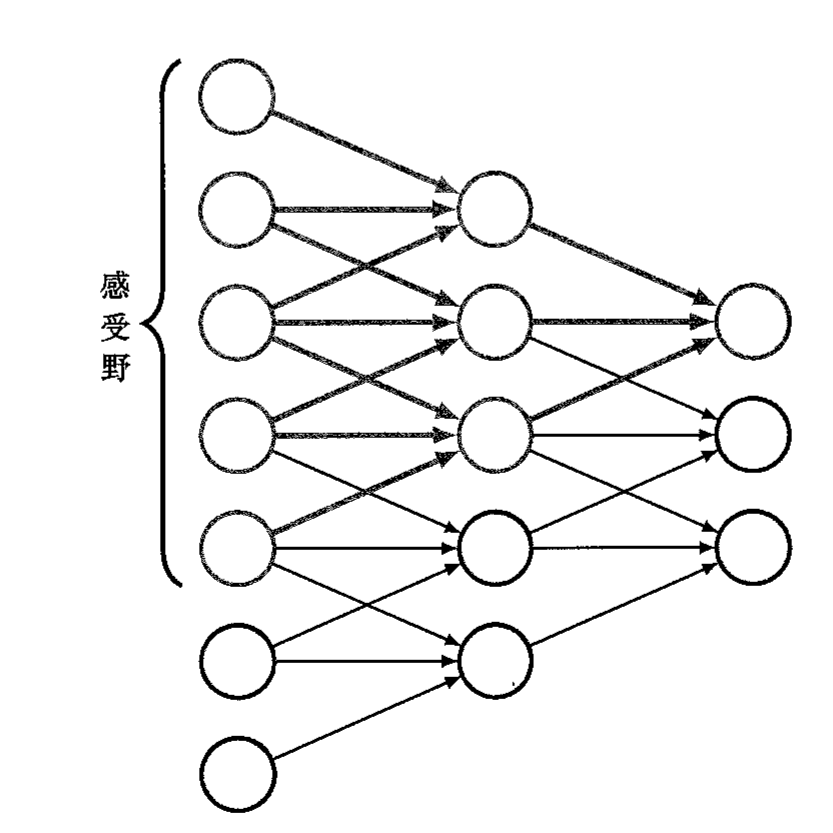
\includegraphics[width=0.55\textwidth]{ch10-fig10-9-有效感受野.png}
  \caption{多层卷积网络中有效感受野如何随深度的增加而增大的示意图。在这里，我们看到输出层顶部的红色单元从中间层单元的感受野中获取输入，每个中间层单元在第一层单元中都有一个感受野。因此，输出层中红色单元的激活取决于中间层中 3 个单元的输出以及输入层中的 5 个单元的输出。}
  \label{figure:ch10-有效感受野}
\end{figure}

早期的 CNN 通常具有较少的卷积层，因为它们具有较大的感受野。例如，AlexNet（Krizhevsky, Sutskever, and Hinton, 2012）具有步幅为 4、尺寸为 $11\times 11$ 的感受野。从\cref{figure:ch10-有效感受野}中可以看出，通过使用每层只有较小感受野的多层结构，也可以隐式地实现较大的感受野。后者的优点是需要的参数要少得多，并且有效地对较大的滤波器施加了归纳偏置，因为它们必定由卷积子滤波器组成。尽管这是一个高度复杂的架构，但只需要对网络函数本身进行显式编码即可，因为我们可以使用自动微分（参见\cref{section:ch08-自动微分法}）来计算损失函数的导数，并使用随机梯度下降来优化损失函数。

在许多应用中，网络的输出单元需要预测图像整体的信息。例如在图像分类任务中，网络需要组合来自整个输入图像的信息。这通常是通过在网络的最后阶段引入一个或两个标准的全连接层来实现的，其中每个单元都连接到前一层中的每个单元。这种架构中的参数数量是可控的，因为中间池化层的存在，最终卷积层的维度通常比输入层的维度少得多。然而，即使网络中（共享的）连接数量比卷积层中的多，最终全连接层也可能包含网络中大多数独立自由度。因此，一个完整的 CNN 包括多层卷积，这些卷积穿插着池化操作，并且通常在网络的最后阶段有传统的全连接层。在设计这样的架构时，需要做出许多选择，包括层数、每层中的通道数、滤波器尺寸、步幅大小以及多个其他此类超参数。在实践中，训练每个候选配置的计算成本很高，很难使用留出法对超参数的值进行系统的比较，研究人员为此探索了各种不同的架构。

\subsection{网络架构示例}\label{subsection:ch10-网络架构示例}

卷积网络是第一个成功部署在应用中的深度神经网络（即具有两个以上可学习参数层的神经网络）。一个早期的例子是 LeNet，它用于对低分辨率的单色手写数字图像进行分类（LeCun et al., 1989; LeCun et al., 1998）。通过引入名为 ImageNet（Deng et al., 2009）的大规模基准数据集，开发更强大的卷积网络得到了加速。该数据集包含约 1 400 万幅自然图像，其中每幅图像都被手工归为近 22 000 个类别之一。这是一个比我们以前使用的所有数据集都大得多的数据集，ImageNet 推动的领域进步强调大规模数据以及设计具有适当归纳偏置的良好模型在构建成功深度学习方案时的重要性。

ImageNet 中包含 1 000 个非重叠类别的图像子集构成了年度 ImageNet 大规模视觉识别挑战赛（ImageNet Large Scale Visual Recognition Challenge）的基础。同样，这比之前通常考虑几十个类别要多得多。拥有如此多的类别使问题变得更加棘手，因为如果类别分布均匀，随机猜测的错误率将达到 $99.9\%$。该数据集包含超过 128 万幅训练图像、5 万幅验证图像和 10 万幅测试图像。分类器旨在为测试图像生成预测输出类别的排序列表，并根据 Top 1 和 Top 5 的错误率报告结果。这意味着如果真实类别出现在列表顶部或位于 5 个排名最靠前的类别预测之中，则视为图像分类正确。该数据集的早期结果实现了 Top 5 的错误率约为 $25.5\%$。AlexNet 卷积网络架构（Krizhevsky, Sutskever, and Hinton, 2012）取得了重要进展，赢得了 2012 年的比赛，并将 Top 5 的错误率降低到 $15.3\%$ 的新纪录。AlexNet 模型的关键之处在于使用 ReLU 函数作为激活函数、应用 GPU 训练网络以及使用 dropout 正则化（参见\cref{subsection:ch09-dropout}）。该模型随后几年取得了进一步的成功，错误率降低至约 $3\%$，在某些数据上，比人类水平（约 $5\%$）表现得要好一些（Dodge and Kara, 2017）。这可以归因于人类难以区分只有微妙差异的不同类别（例如不同的蘑菇品种）。

作为典型卷积网络架构的一个示例，我们来详细了解一下 VGG-16 模型（Simonyan and Zisserman, 2014），其中 VGG 代表开发该模型的 Visual Geometry Group，16 表示模型中可学习层的数量。VGG-16 模型有一些简单的设计原则，旨在得到相对一致的架构，如\cref{figure:ch10-VGG16架构}所示，即最大限度地减少需要选择的超参数的数量。

\begin{figure}[htbp]
  \centering
  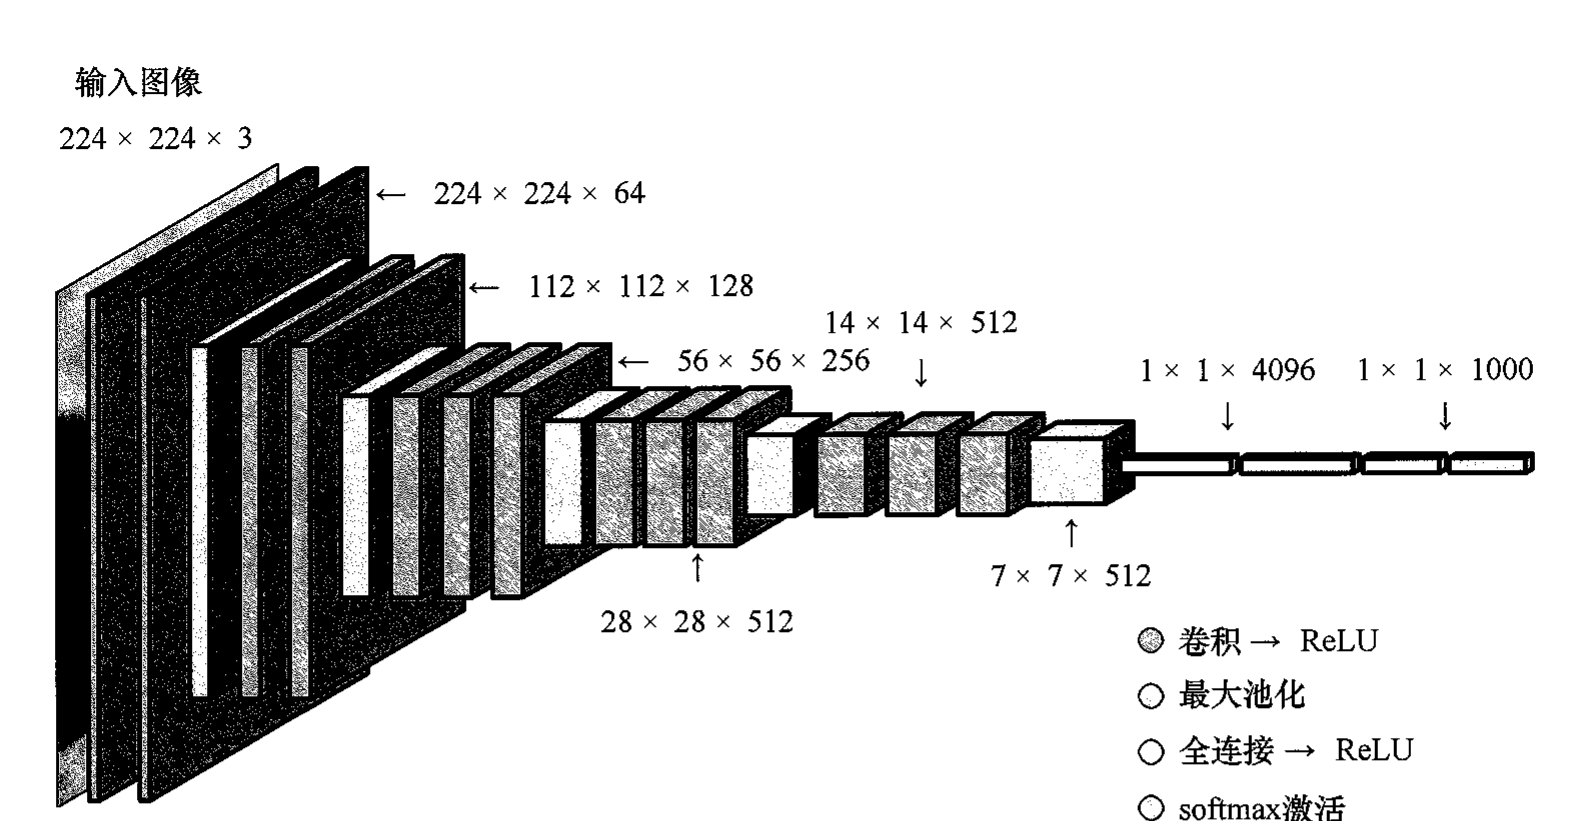
\includegraphics[width=0.95\textwidth]{ch10-fig10-10-vgg16.png}
  \caption{一个典型卷积网络（在本例中是 VGG-16 模型）的架构。}
  \label{figure:ch10-VGG16架构}
\end{figure}

该模型以 $224\times 224$ 像素和三颜色通道的图像作为输入，然后接入穿插有下采样的卷积层集合。所有卷积层都具有尺寸为 $3\times 3$、步幅为 1 的滤波器，执行等大填充并使用 ReLU 激活函数；而最大池化操作都使用步幅为 2、尺寸为 $2\times 2$ 的滤波器，从而将单元数下采样为原先的四分之一。第 1 个可学习层（简称第 1 层）是一个卷积层，其中每个单元从输入通道堆叠得到的 $3\times 3\times 3$ 的“立方体”获取输入，因此包括偏置在内共有 28 个参数，这些参数在该通道的特征图中的所有单元之间共享。第 1 层有 64 个这样的特征通道，从而使输出张量的大小为 $224\times 224\times 64$。第 2 层也是卷积层，同样有 64 个通道。紧接着是最大池化层，给出的特征图大小为 $112\times 112$。第 3 层和第 4 层又是卷积层，维度为 $112\times 112$，每层都有 128 个通道。通道数量的增加在一定程度上抵消了最大池化层中的下采样，以确保每层表示中的变量数量不会随着所通过网络层数的增加而过快地减少。同样，接下来是最大池化操作，以产生大小为 $56\times 56$ 的特征图。接下来是另外三个卷积层，每个卷积层有 256 个通道，从而再次将与下采样相关的通道数量增加一倍。接下来是另一个最大池化操作，得到大小为 $28\times 28$ 的特征图。紧接着又是三个卷积层，每个卷积层有 512 个通道，后面跟着另一个最大池化操作，下采样得到大小为 $14\times 14$ 的特征图。接下来是另外三个卷积层，尽管这三个卷积层中的特征图数量保持在 512，但接下来再次进行最大池化操作，从而将特征图的大小减小到 $7\times 7$。最后，还有三层是全连接层，这意味着它们是具有完全连接且不共享参数的标准神经网络层。最终的最大池化层有 512 个通道，每个通道的大小为 $7\times 7$，总共 25 088 个单元。第一个全连接层有 4 096 个单元，每个单元都连接到每个最大池化单元。接下来是第二个全连接层，它同样有 4 096 个单元。最后是第三个全连接层，它有 1 000 个单元，以便将网络应用于包含 1 000 个类别的分类问题。网络中除输出层外的所有可学习层都具有非线性 ReLU 激活函数，输出层具有 softmax 激活函数。

总体而言，VGG-16 模型中总共有大约 1.38 亿个可独立学习的参数，其中大部分（近 1.03 亿个）位于第一个全连接层中，而大多数连接位于第一个卷积层中（参见\cref{exercise:ch10-08}）。

\begin{example}[ VGG-16 的逐层参数量]\label{example:ch10-VGG16参数}
按\cref{proposition:ch10-卷积层参数量}逐个计算 VGG-16 的参数。13 个卷积层的参数依次为
\begin{align*}
  &(3\cdot3\cdot3+1)\cdot64=1\,792, &&(3\cdot3\cdot64+1)\cdot64=36\,928,\\
  &(3\cdot3\cdot64+1)\cdot128=73\,856, &&(3\cdot3\cdot128+1)\cdot128=147\,584,\\
  &(3\cdot3\cdot128+1)\cdot256=295\,168, &&2\times\bigl[(3\cdot3\cdot256+1)\cdot256\bigr]=1\,180\,160,\\
  &(3\cdot3\cdot256+1)\cdot512=1\,180\,160, &&5\times\bigl[(3\cdot3\cdot512+1)\cdot512\bigr]=11\,799\,040,
\end{align*}
三个全连接层分别为 $7\cdot7\cdot512\cdot4096+4096=102\,764\,544$、$4096\cdot4096+4096=16\,781\,312$ 与 $4096\cdot1000+1000=4\,097\,000$。
\end{example}

\begin{proposition}[VGG-16 的总参数量]\label{proposition:ch10-VGG16参数量}
按\cref{figure:ch10-VGG16架构}的结构（13 个卷积层、3 个全连接层、池化层无可学习参数），VGG-16 的可学习参数总数为
\begin{align}
  N_{\mathrm{VGG16}}=138\,357\,544\approx1.38\times10^{8},
  \label{align:ch10-VGG16参数量}
\end{align}
其中第一个全连接层贡献 $102\,764\,544$ 个参数，约占总数的 $74\%$。
\end{proposition}
\begin{proof}
卷积层部分由\cref{example:ch10-VGG16参数}逐层相加：
\begin{align*}
  &1\,792+36\,928+73\,856+147\,584+295\,168+1\,180\,160+1\,180\,160+11\,799\,040\\
  &\quad=14\,714\,688 .
\end{align*}
全连接层部分为 $102\,764\,544+16\,781\,312+4\,097\,000=123\,642\,856$。故总数为 $14\,714\,688+123\,642\,856=138\,357\,544$。第一个全连接层所占比例为 $102\,764\,544/138\,357\,544\approx0.743$，即约 $74\%$。证毕。
\end{proof}

% SUPPLEMENT: parent=proposition:ch10-VGG16参数量; kind=motivation; location=紧随其后的 remark（重构新增）
\begin{remark}（重构新增）
这个计算说明了一个反直觉的事实：VGG-16 的绝大多数参数并不在卷积层，而在最后三个全连接层，因为 $7\times7\times512$ 与 $4096$ 之间的全连接矩阵没有任何权重共享。由此可以理解后续架构（如 ResNet）为何用全局平均池化取代大全连接层：不是为了减少连接，而是为了减少独立自由度。计算时逐层核对三件事：输入通道数是否等于上一层的输出通道数、$3\times3$ 卷积是否保持空间尺寸（等大填充，$P=1$）、池化是否把边长减半。若把某个 $3\times3$ 卷积误当作 $5\times5$，或漏掉偏置，总数就会偏离 $1.38$ 亿；因此这个数字可以作为架构描述的校验和。注意题目所说的“权重数量（连接数）”与“独立可学习参数”是两个不同的量，前者还要乘以输出特征图的空间尺寸，后者与 $J,K$ 无关。
\end{remark}

\end{document}
